%!TEX root = ../main.tex
\chapter{Dioden Modelle }
Besteht bei einem elektrischen Bauteil ein linearer Zusammenhang zwischen Ursache (Eingang) und Wirkung (Ausgang), spricht man von einem Linearen Bauteil. Die  U-I-Kennlinie stellt eine Geradengleichung dar. Lineare Bauteile und Schaltungen aus linearen Bauteilen lassen sich durch einfache Methoden berechnen. 
Die Diode ist kein lineares Bauelement, die U-I-Kennlinie lässt sich nicht ohne weiteres berechnen. Um die Kennlinie einer Diode näherungsweise zu beschreiben, wurden unterschiedliche Dioden Modelle eingeführt. 

\section{Die Ideale Diode}
Bei einer Idealen Diode geht man davon aus, das sie in Durchlassrichtung keinen ohmschen Widerstand besitzt und in Sperrrichtung einen unendlich großen ohmschen Widerstand aufweist. Bei dieser sehr groben Näherung kann man die Diode als idealen Schalter betrachten.

\begin{figure}[!htb]
\centering
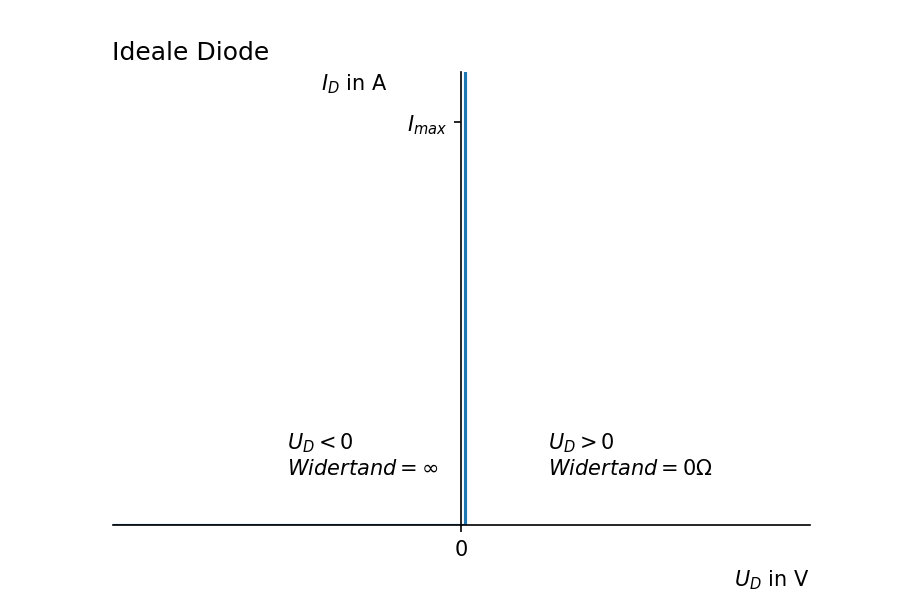
\includegraphics[scale=0.8]{IdealeDiode.png}
\caption{I-U Kennlinie einer Idealen Diode (matplotlib)}
\end{figure}

\section{Konstantspannungs-Diode}
Bei diesem Modell wird die Schleusenspannung berücksichtigt. Wie in dem Kapitel \ref{sec:DiodeInDurchlassrichtung} beschrieben, fließt durch die Diode in Durchlassrichtung erst ein nennenswerter Strom, wenn die Äußere Spannung $U_{S}$ größer ist als die innere Diffusionsspannung $U_{D}$. Dies wird in der Kennlinie der Idealen Diode durch das verschieben nach rechts zur Schleusenspannung $U_{S}$ ersichtlich. 

\begin{figure}[!htb]
\centering
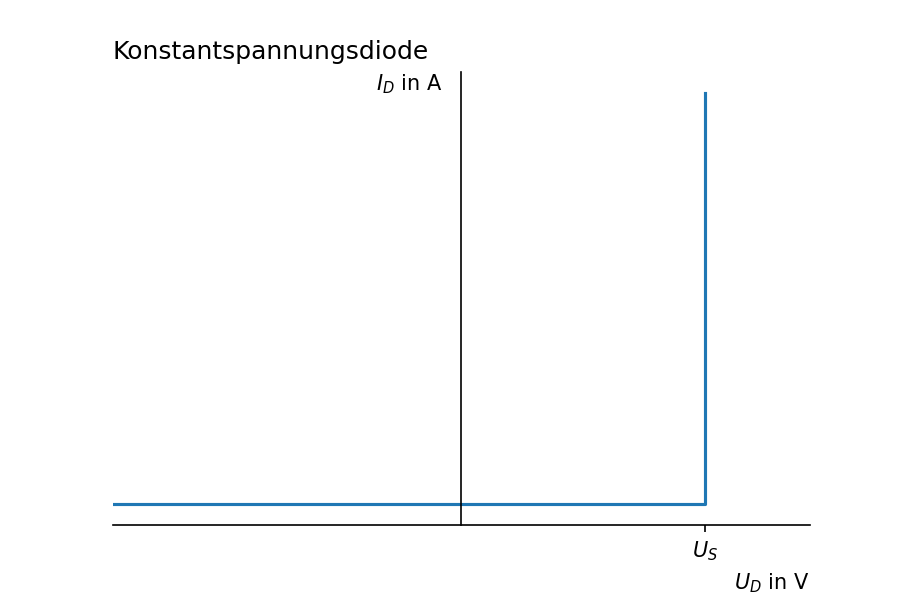
\includegraphics[scale=0.8]{KonstantSpannungsDiode.png}
\caption{I-U Kennlinie einer Konstantspannungs-Diode (matplotlib)}
\end{figure}



\section{Konstantspannungs-Diode mit Bahnwiderstand}

In diesem Model wird berücksichtigt, dass die Diode auch nach dem Überschreiten der inneren Diffusionsspannung ein Widerstand aufweist. Somit steigt die gesamt Spannung der Diode bei zunehmenden Strom an. Berücksichtigt wird dabei der Widerstand der elektrischen Kontaktierung und der Widerstand vom Bahnbereich (Kapitel\,     \ref{sec:Aufbau einer Halbleiter Diode}) 

\begin{figure}[!htb]
\centering
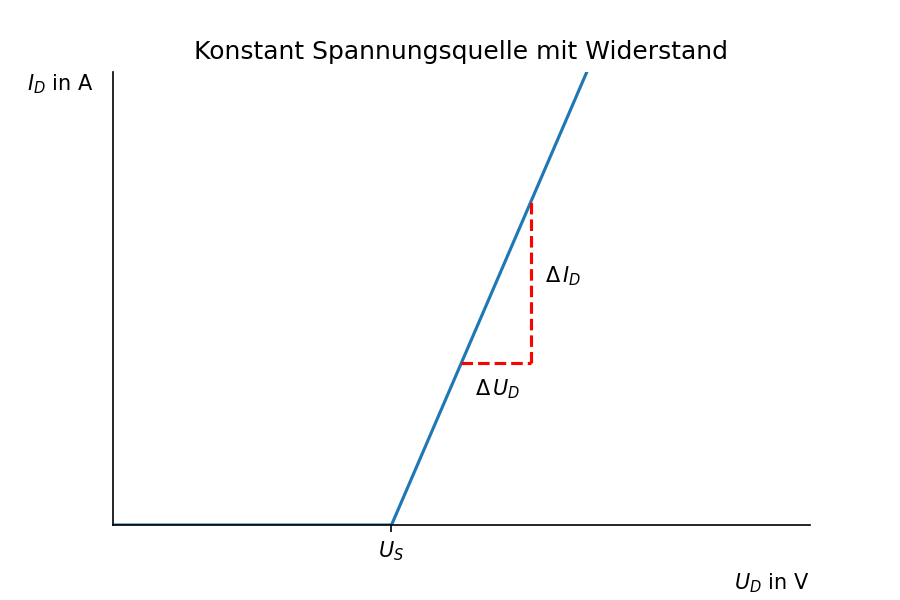
\includegraphics[scale=0.8]{KonstSpannungWiderstand.png} 
\caption{I-U Kennlinie einer Konstantspannungs-Diode mit Widerstand (matplotlib)}
\end{figure}

\newpage
\section{Shockley Diode}

Die Shockley Gleichung \eqref{eq:shockley} ermöglicht es die I-U Kennlinie einer Idealen Diode zu beschreiben. 

\begin{figure}[!htb]
\begin{equation}
I_{D} (U_{D}) = I_{S} \cdot \left(e^{\frac{U_{D}}{U_{T}}}-1\right)
\label{eq:shockley}
\end{equation}
\begin{align*}
I_{D}(U_{D}) &= \text{Strom durch die Diode in Abhängigkeit der Spannung an der Diode}\\
U_{D} &= \text{an die Diode angelegte äußere Spannung}\\
I_{s} &= \text{Sperrsättigungsstrom ein Datenblattwert ca $10^{-14}\ldots 10^{-6}A$}\\
e &= \text{Eule'rsche Zahl}\\
U_{T} &= \text{Temperaturspannung bei Raumtemperatur $T = 300K $ ist $U_{T} \approx 26mV$ }
\end{align*}
\end{figure}

\begin{figure}[!htb]
\begin{equation}
U_{T} = \dfrac{k \cdot T}{e}
\label{Temperaturspannung}
\end{equation}
\begin{align*}
k &= \text{Boltzmann-Konstante $= 1,380658 \cdot 10^{-23} \scriptstyle \frac{K}{J}$} \\
T &= \text{absolute Temperatur der Sperrschicht in Kelvin}\\
e &= \text{Betrag der Elementarladung $= 1.6 \cdot 10^{-19}C$}
\end{align*}
\end{figure}
\begin{figure}[!hbt]
\centering
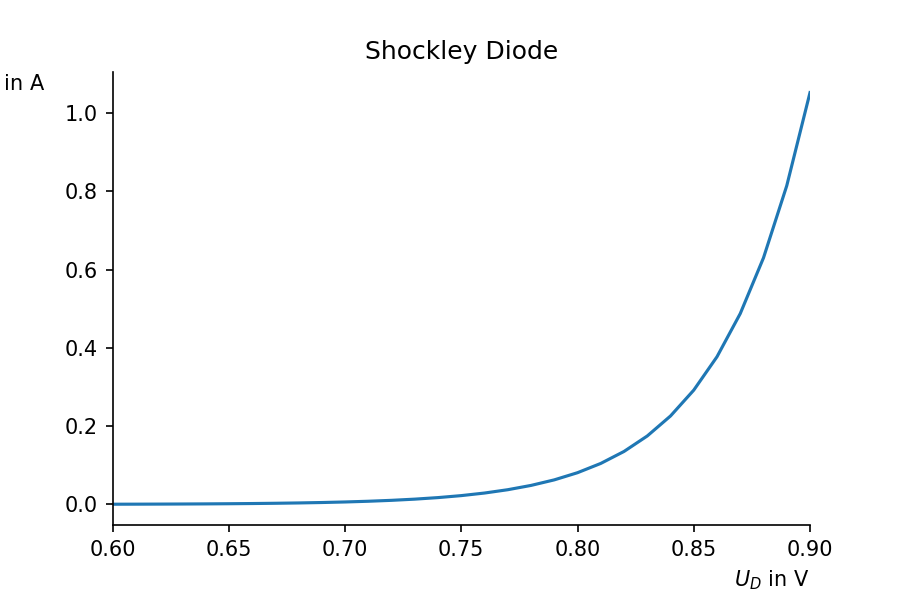
\includegraphics[scale=0.8]{Shockley.png}
\caption{Shockly Diode}
\end{figure}
